%\tableofcontents


\section{Introduction}
\label{section:Introduction}
Interactive data analysis requires the user to interact with and explore the data to better understand it. The use cases for this are rapidly increasing, leading to a greater need for new design space interaction techniques that enable intuitive and effective interaction with abstract high-dimensional data. While 2D space visualisation can make use of a direct mapping from interaction space to display space, immersive environments also need to consider the context of the setup and the task to be solved. Either way visualization is the key part for humans to understand large and complex data sets \autocite[]{Donalek2015}. \newline
Recent approaches try to further explore tangible interfaces, which compared to traditional desktop setups allow a higher \ac{DOF} \autocite{Bach2018} \autocite[]{Besancon2017} and \ac{HMD}s, that lead to a better sense of stereoscopic depth and perception. The use of \ac{HMD}s is connected to \ac{VR} or \ac{AR} environments, often also called mixed or extended realities, where compared to traditional 2D desktop settings a more natural interaction is possible. As \cite{Bach2018}'s research shows, combining immersive environments with tangible user interfaces appears to be a potentially effective approach for interacting with multidimensional data visualisations.\newline
Immersive visualization can be described as the field of visualizing information in immersive environments such as \ac{VR} or \ac{AR}. This not only leads to improved effectiveness of the data visualisations, but also allows the user to explore it in a more intuitive way and speeds up pattern finding [\autocite[3]{Butscher2018}, \autocite[489]{WagnerFilho2018}]. Use-cases vary a lot, where commonly used visualisation methods are 3D scatter plots or graph visualisation. However, also new approaches are explored e.g. flexible axes arrangement \autocite[]{Cordeil2017a} and proven to be useful for certain tasks due to a higher \ac{DOF}.\newline
Compared to 2D visualisation, high-dimensional immersive visualizations try to overcome typical problems of occlusion, perceptual distortion or misleading correlation of data. Immersive environments distinguish between the interaction-space, usually the user's real environment and the display-space, where the actual visualisation is presented in a virtual context. Designing interaction mapping from these two spaces remains a challenge.\newline
This paper analyses and evaluates already existing possibilities for immersive visualisations starting by discussing different setup scenarios and data visualisations methods. It continues to analyse interaction techniques, that can potentially be as effective, as mouse and keyboard interaction techniques in 2D space. Typically there are three types of interaction issues in 3D space: Navigation \& Movement, Selection \& Manipulation and System Control, to which it will be referring. 
Interaction implementations in immersive environments are then discussed in terms of their input techniques used. 
To conclude, the paper presents some Open-Source tool-kits and examples for immersive data visualisations and how they solve interaction issues in \ac{AR} or \ac{VR}.

\section{Immersive Visualization Methods}
\label{section:ivm}
There are many different data visualisation methods. The most common are 3D scatterplots or graph visualisations. 3D scatterplots in combination with \ac{VR} setups overcome issues such as over-plotting or occlusion by providing new ways of interacting with it \autocite[]{Prouzeau2019}. These scatterplots use three quantitative attributes of the data and map them to display space. But when it comes to high density regions they are inefficient and need further optimization \autocite[]{Prouzeau2019}.
For high-dimensional data, it is common to use \ac{DR} to create a reduced version of the data with the same characteristics, which can then be displayed in 3D scatterplots as shown in Fig. \ref{figure:DR3DScatterplots} \autocite[484]{WagnerFilho2018}.
\begin{figure}[!ht]
    \centering
	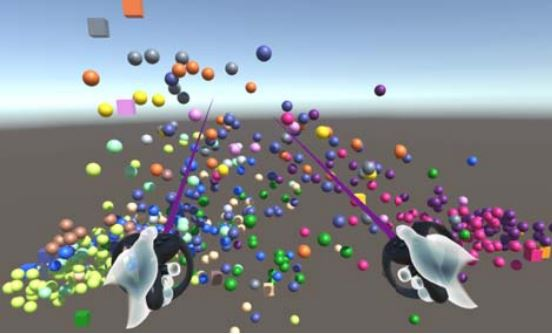
\includegraphics[width=0.5 \textwidth]{images/Filho2020_controllers_interaction_scatterplots.jpg}
	\caption{
		Exploration of \ac{DR} data scatterplots in HMD-based immersive environments \autocite{WagnerFilho2018}.
	}
	%for reference to this figure
	\label{figure:DR3DScatterplots}
\end{figure}
\newline\cite[]{Kwon2016} investigated spherical graph layouts, in which the user's \ac{FOV} is placed at the center of the sphere (Fig. \ref{figure:SpericalGraphCenteredView}) to reduce the spatial navigation overhead. A challenge in graph visualisations is dealing with the large set of edges, which is addressed by routing the edges around the surface of the sphere \autocite[1803]{Kwon2016}.
\begin{figure}[!ht]
    \centering
	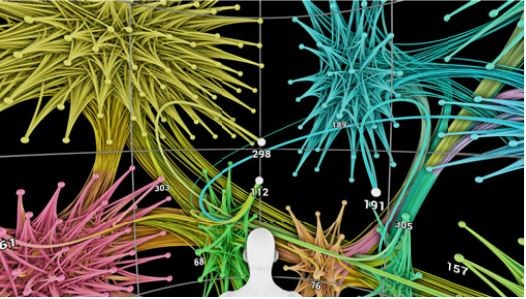
\includegraphics[width=0.49 \textwidth]{images/Kwon2016_sphericalgraphlayout_centereduser.jpg}
	\caption{
		The user's view is centered in the spherical graph visualisation  \autocite{Kwon2016}.
	}
	%for reference to this figure
	\label{figure:SpericalGraphCenteredView}
\end{figure}
ImAxes uses a grammar-based approach to construct the visualisations with spatial placement of data axes. The user is then allowed to build upon grammar rules and combine them in any way he likes. The only restrictions are, that the different axes must be touching and either parallel or orthogonal to the other axes \autocite[]{Cordeil2017a}. This allows the user to decide whether they want to see a histogram, a scatterplot or more complex visualization views. ImAxes is limited by the number of axes used as well as by the size of the data set, as these affect the smooth interaction and performance of the visualization.
\begin{figure}[!ht]
    \centering
	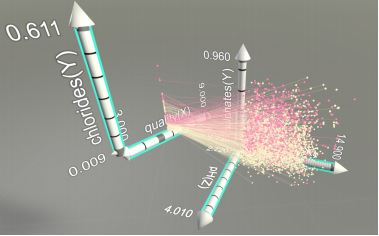
\includegraphics[width=0.49 \textwidth]{images/Cordeil_ImAxes.jpg}
	\caption{
		Possible axes arrangement with data visualisation using ImAxes \autocite{Cordeil2017a}.
	}
	\label{figure:ImAxes}
\end{figure}
\section{Hardware}
\label{section:hardware}
This paper will focus on two platforms for immersive visualization as they are widely available: \ac{HMD}s and tablets. Alternative setups are desktop setups or CAVE systems, but are not focus of this work.

\subsection{Head-Mounted Displays}
\label{subsection:hmd}
\ac{HMD}s offer high-resolution displays and accurate, low-latency head-motion tracking, as well as stereo vision depth, greatly enhancing human perception in 3D space \autocite[46]{Cordeil2017}. 
Because those displays are placed directly in front of the user's eyes, only the user's view needs to be rendered and thus can be controlled easily \autocite[1802]{Kwon2016}.
Furthermore, the use of \ac{HMD}s invites to embodied navigation, as the user can move around and change their viewpoint without losing sight of data. Handheld controllers such as the HTC Vive controller \footnote{https://www.vive.com/us/accessory/controller/} or free hand gestures with a leap motion controller \footnote{https://www.ultraleap.com/product/leap-motion-controller/} or the Microsoft Kinect are most commonly used for interaction tasks.\newline
A possible \ac{HMD} is the Microsoft Hololens \footnote{https://www.microsoft.com/en-gb/hololens} - a lightweight see-through AR headset for usage on the PC and the AR view \autocite[]{Wang2020}.
Technical shortcomings include a limited \ac{FOV} and low display resolution, but will be removed in future hardware \autocite[]{Wang2020}. Compared to other hardware, \ac{HMD}s not only enhance the sense of presence in the immersive environment with proper tracking, but also enable interaction with both the virtual and real word.\newline

\subsection{Tablets}
Tablets are a broadly used alternative to \ac{HMD}s, as they offer both tangible and tactile input and are capable of tracking their own position in 3D space. On \ac{TUI} the interaction space and the display space can be integrated on the same device. However, they can also be used for processing only interaction input and the display is done on a separate device.\newline Tactile input benefits from its directness, precision and rich feedback, whereas accuracy of interaction can be an issue with finger fatigue. With a minimum of 6 \ac{DOF}, tangible interaction uses advantages of users natural skills for manipulating physical object \autocite[881-882]{Besancon2017}. \newline
\ac{TUI}s use a direct mapping from interaction to the visualizations and are designed to support navigation, selection, and menu interaction [\autocite[47]{Cordeil2017},\autocite[4]{Butscher2018}]. Users report them to be more engaging then other interactions devices, because they aim to use their natural abilities to manipulate objects. Although, they have problems with accuracy and interaction tasks such as zooming to navigate \autocite[882]{Besancon2017}. \newline
In general, a limitation of tablets compared to \ac{HMD}s is, that they do not allow the user move freely and thus interact in a room-sized design space. In addition, one must consider that the need to hold the tablet while interacting prevents the user from interacting with both hands \autocite[883]{Besancon2017}.

\section{Interaction Techniques Overview}
\label{section:Interaction Techniques 3D}
Interaction with visualizations in immersive environments is still an issue and needs further research. 2D interaction devices such as the mouse or touchscreens allow very precise control by directly mapping from physical space to the virtual data space \autocite[1]{Cordeil2017}. Interaction in 3D space is important for exploring dense data sets, but requires a higher degree-of-freedom \autocite[]{Bach2018}. It should also be remembered, that these are dependent on the setup used. The challenge is to design enjoyable interaction techniques with precise mapping \autocite[]{Jankowski2013}. Typical interaction tasks in immersive environments can be categorised into three areas: Navigation \& Movement, Selection \& Manipulation and System Control. In the next chapters, this paper summarizes existing interaction techniques, that can be assigned to one of the previously mentioned fields.

\subsection{Navigation and Movement}
\label{subsection:Navigation}
Navigation means changing the user's perspective on the display space relative to the interaction space by rotating, translating and scaling \autocite[48]{Cordeil2017}. In desktop visualisations the two most established techniques are zooming in or out to gain more or less details of a region, and providing a minimap window that constantly shows all the data \autocite[1214]{Yang2021}. In immersive environments, the most obvious approach to navigate is physical movement. This reaches its limits in setups that do not allow movement or are limited to the size of the room.\newline Teleportation is another common technique to navigate through space in \ac{VR} settings by ray casting to a desired location in visualisation space using a tracked controller. Whereas drag-and-drop teleportation gives the user more control over their position and orientation, point-and-click teleportation requires fewer steps but may not achieve as accurate results. In general, teleportation seems to be a preferred technique by users, as it requires less effort, reduces the amount of collisions and increases speed \autocite[2]{Drogemuller2020}.\newline\ac{WIM} is the equivalent to the minimap used in desktop visualisations, for always keeping an overview of the data and the possibility to move quickly to a specific location \autocite[1214]{Yang2021}. One of the main issues to be solved with that technique is the placement of the minimap, because it should be constantly present on the one hand, but on the other hand it should not distract the user or lead to unwanted occlusions. \newline
\ac{OHF} or \ac{THF} are other navigation techniques that measure the user`s pointing in a direction and also take into account the time duration of pointing, i.e. the longer the user extends his arm in a certain direction, the faster he travels. During the duration of travel, it is common to fix the user's \ac{FOV} to a specific point to reduce discomfort and motion sickness \autocite[2]{Drogemuller2020}.

\subsection{Selection and Manipulation}
\label{subsection:Selection and Manipulation}
Since users want to interact in with the data, object selection and manipulation is an important component. Existing selection techniques for 3D object in virtual environments use ray-casting to pick or point at them, which is highly prone to error in the absence of an explicit 3D shape\autocite[1]{Yu2016}. One problem that arises with structure-aware-selection techniques that use a 2D lasso drawn on the 3D projection is, that the user must first select a good view for the selection interaction, which can be problematic in complex data sets \autocite[1]{Yu2016}. Therefor, \cite{Yu2016} developed context-aware selection techniques (CAST), which attempt to infer the user's subtle selection intent from gestural input, and was found to be faster and more flexible than other interaction techniques. Moreover, it is not limited to mouse or pen-based input \autocite{Yu2016}.

\subsection{System Control}
\label{subsection:System Control}
Compared to selection and navigation interactions, which take place in the interaction space, system control needs further commands that can be more related to the display space \autocite[48]{Cordeil2017}. It can be referred to as the user-system communication, as those commands change the state of the application \autocite[]{Jankowski2013}.
Menus for common tasks such as switching modes, setting parameters, or selecting a data set should be easily accessible to the user. That is why they are often placed in a corner or the top, so that they are constantly on the interface \autocite[885]{Besancon2017}. Other system control tasks may consist of allowing the user to enable or disable various input modalities or settings. Shortcuts are commonly used to efficiently access system control functions via menu items or icons \autocite[]{Jankowski2013}. \newline

\section{Interaction In Immersive Visualisations}
Interaction methods to interact with immersive visualisations are hardly explored, but a key part for data exploration. This paper analyses some of them based on their input system.
\label{section:Interaction Techniques Immersive}

\subsection{Mouse-based Interaction}
\label{subsection:Desktop-based Interaction}
Since people today are used to working on desktop-setups with mouse and keyboard, this is still often used to interact with data visualisations. 
 \cite{Wang2020} designed a system that uses mouse and keyboard input, as previous work pointed out that scientists prefer to use well-know interaction techniques over novel and even more effective ones. Reasonable as mouse and keyboard offer high precision, which is important for data analysis. 
 \newline \cite{Kwon2016} found that for selection tasks in his graph-based study controlling the cursor via mouse input relative to the fixed spherical space is most effective. The issue of the cursor leaving the user's \ac{FOV} was solved by displaying an arrow pointing at the cursor's position and a shortcut for resetting its position \autocite[]{Kwon2016}.
In the comparison study of \cite{Bach2018}, the desktop environment with mouse interaction also recorded high precision.

\subsection{Tablet-based Interaction}
\label{subsection:Tablet-based Interaction}
The rich feedback and accuracy of touch and tangible input on tablets can be used for user data interaction. \cite{Besancon2019} developed a Tangible Brush technique for selecting regions of interests in the data. Therefor the user must first draw a closed shape on the tablet display (2D lasso), which is then extended into 3D space. After that, the user can move the tablet in physical space to brush through the data and finalise the selection. Compared to CAST techniques \autocite{Yu2016} it resulted in being very accurate but slower.\newline
Spatial interaction is another approach, that takes the advantage of the tablet's position and orientation tracking capability to navigate data sets. Compared to touch input, participants in this study preferred spatial interaction because it was more supportive and comfortable to use \autocite{Buschel2017}. For filtering and selection tasks, however, the touch input is still used and needed.

\subsection{Controller-based Interaction}
\label{subsection:Controller-based Interaction}
The use of \ac{HMD}s is usually accompanied by the use of hand-held controllers for interacting in immersive environments. As discussed in section \ref{subsection:Navigation}, teleportation is commonly used to move around and change the perspective on the data, which is triggered by interaction with the controllers.\newline Hand-held controllers are used by \cite{Cordeil2017a} to scale and filter the data axes. Therefore widgets are animated out of the according axes and respond to the interaction, which gives continuously feedback.\newline
Scaptics and Highlight-Plane (Fig.\ref{figure:HighlightPlane}) are alternative interaction techniques for exploring hidden features in 3D scatterplots. Scaptics (Scatterplot Haptics) integrates haptic feedback to HTC Vive handheld controllers by mapping density information in the data to vibration on the controller. Highlight-Plane uses a cutting-plane to enable the user to explore density and spatial arrangement of data as shown in Fig. \ref{figure:HighlightPlane} \autocite[]{Prouzeau2019}.
 \begin{figure}[!h]
    \centering
	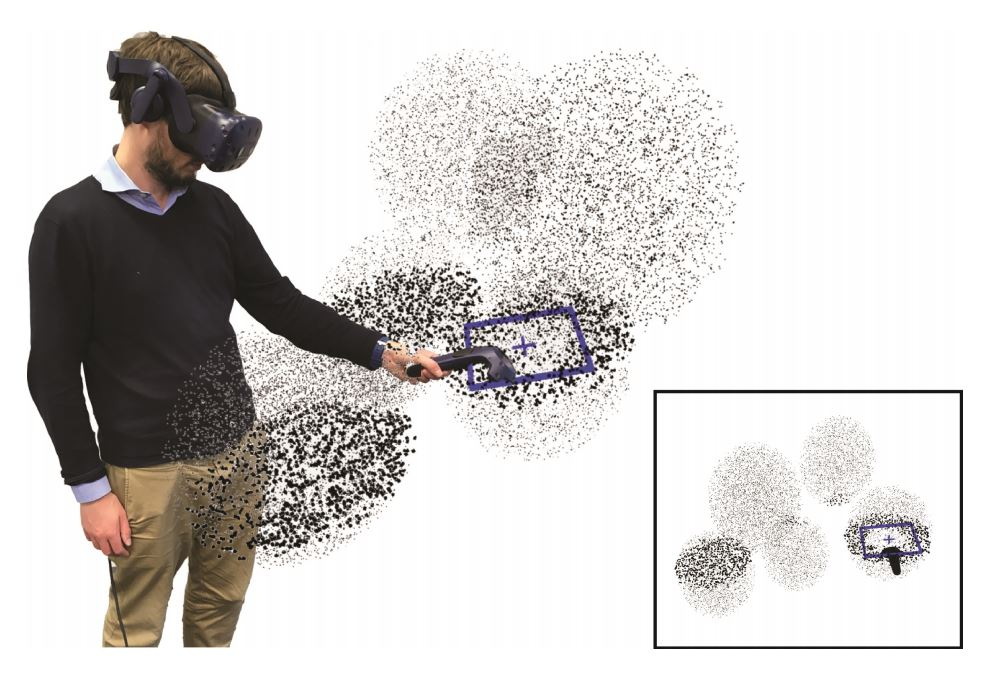
\includegraphics[width=0.5 \textwidth]{images/Prouzeau2019_HighlightPlane.JPG}
	\caption{
		Highlight Plane technique  \autocite{Prouzeau2019}
	}
	\label{figure:HighlightPlane} 
\end{figure}

\subsection{Gesture-based Interaction}
\label{subsection:Gesture-based Interaction}
The most natural input for interacting with data visualizations in immersive environments seems to be gestures, but interaction detection and interpretation is a difficult problem to solve, so that it is not as effective as expected.\newline
\cite{Cordeil2017b} used a Leap Motion controller tracked on the top of a \ac{HMD} to allow natural gestures as input. Participants in his collaborative study complained about issues when the controller could not track the position of the fingers because they were out of sight.\newline
Also \cite{Clarke2016} used the Leap Motion controller to track the user's hand position and orientation for interacting with a time-dependent graph visualised in a cube. Rotation is possible by rotating a smaller instance of the cube, where feedback is given through the real time rendering of the cube and the mapping of the user's hand from real into virtual world.\newline
Another possible input device for gestures is the Microsoft Kinect, which was used in the study of \cite{Nagao2017}. Interaction contained pressing virtual buttons, changing values in sliders on the \ac{HMD} interface or physically moving the open hand to rotate the data images.\newline
Using a hand-tracked interface for exploring microscopy data leads to higher productivity \autocite[]{Theart2017} and lower cognitive load \autocite[]{Filho2020}, despite side effects of inaccuracy and frustration. 
A recent study for object selection in dense immersive visualisations showed, that a point and tap gesture works best for participants \autocite[]{Bhowmick2021}. \newline

\subsection{Tangible Interaction}
\label{subsection:TangibleInteraction}
A more novel approach is interaction via tangible objects e.g. markers. \cite{Besancon2017} designed a flexible seed point placement method, where ray-casting as tactile and cutting plane manipulation as tangible input can be used in combination by the user \autocite[885]{Besancon2017}.
\begin{figure}[!ht]%
    \centering
    \subfloat[\centering]{{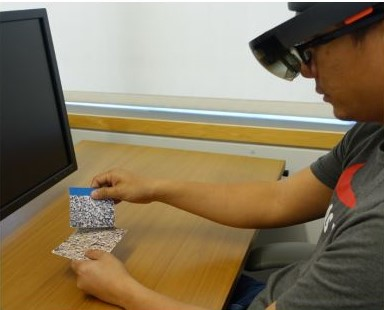
\includegraphics[width=0.4\linewidth]{images/Bach2018_ImmersiveAR_left.jpg} }}%
    \qquad
    \subfloat[\centering]{{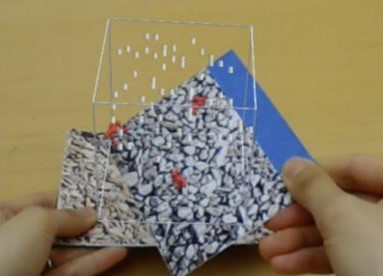
\includegraphics[width=0.45\linewidth]{images/Bach2018_ImmersiveAR_right.jpg} }}%
    \caption{Immersive Tangible AR with the HoloLens and tangible markers \autocite{Bach2018}.}%
    \label{fig:ImmersiveAR}%
\end{figure}
\newline Immersive tangible \ac{AR} - the combination of the HoloLens and tangible fiducial markers - allows the user to place the visualisation wherever he wants. The interaction with tangible markers e.g. a cutting plane technique can improve time and accuracy \autocite[]{Bach2018}. It was at least as precise as interacting with a mouse and can be improved with training. Furthermore, tangible markers provide seamless two-handed interaction in both input and display space \autocite[]{Billinghurst2008}.
 \begin{figure}[!ht]
    \centering
	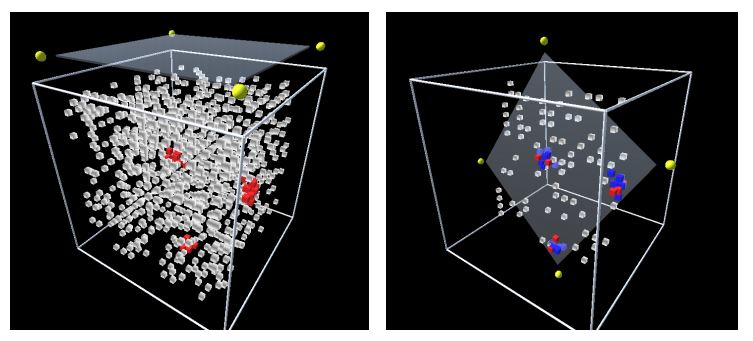
\includegraphics[width=0.5 \textwidth]{images/Bach2018_CuttingPlane-jpg.JPG}
	\caption{
		Cutting plane technique for selecting three data points at the same time \autocite{Bach2018}.
	}
	%for reference to this figure
	\label{figure:CuttingPlane} 
\end{figure}

\section{Tools and Examples}
\label{section:Tools} 
Building applications and tools for immersive visualisations comes with many challenges and often requires domain specific knowledge in the fields of data visualisations, analytics, computer graphics, human-computer-interaction and \ac{AR}/\ac{VR} \autocite[1]{Sicat2019}. Below this paper presents open-source tools, that facilitate the creation process of immersive visualisations.\newline
ART - Augmented Reality above the tabletop uses \ac{AR} \ac{HMD}s to visualize a 3D parallel coordinates plot in a physical space by linking together individual 2D scatter plots and combines it with a touch-sensitive tabletop for interaction. Furthermore, it supports collaborative analysis \autocite[]{Butscher2018}. \newline
DXR - an Unity\footnote{https://unity.com/} based open-source toolkit, that helps to speed up building and prototyping data visualisation applications for eXtended Reality by providing  a higher level interface for constructing and adapting visualisations. Regarding interaction DXR provides scaling up and down, rotating along x, y, z-axis, view configuration controls and can be extended to further device-dependent affordances \autocite[2]{Sicat2019}.\newline
IATK, the Immersive Analytics Toolkit is an open source software package for Unity to facilitate the creation of data visualisations and immersive analytic systems by providing standard routines, predefined visualisations and support for creating novel visualisations and interactions. It uses a grammar of graphics, that is configurable by the user with a GUI \autocite[]{Cordeil2019}.\newline
iViz - a multi platform data visualizer prototype based on Unity includes a broadcasting function, allowing collaborative, multi-user data exploration. It supports the Leap Motion sensor, a 3D mouse and Kinect for interaction and the Oculus Rift \ac{VR} googles as display device. \autocite[]{Donalek2015}\newline
ImAxes - Immersive Axes - is an Unity based immersive visualisation toolkit for exploring multidimensional data visualisations. It relies on the spatial arrangement of data axes, that can be combined and manipulated easily via controller-based interaction \autocite[]{Cordeil2017a}. \newline
VRIA - a web based framework for creating \ac{VR} immersive analytics experiences based on WebVR, A-Frame, React and D3.js. Because of being implemented on web-based technologies, it is accessible everywhere and easy to extend and manipulate via the Document Object Model \autocite[]{Butcher2020}. It supports gaze, controller and touch based interaction methods, but is limited by performance.\newline
MIRIA - a mixed reality toolkit for collaborative in-situ analysis of multidimensional spatial data visualisations using Microsoft HoloLens \ac{HMD}s \autocite[]{Buschel2021}. It supports multiple visualisation views and multiple ways to filter the data. \newline
MARVIS - a framework that combines mobile devices and \ac{AR} using the Microsoft HoloLens \ac{HMD} \autocite[]{Langner2021}. The main interaction is handled via touch input on the mobile device(s) and then visualised in virtual space above the displays on the mobile devices.
\section{Discussion}
As discussed and demonstrated in this paper, a tool or application for interactive data visualisations should provide different interaction techniques depending on the setup used, to allow the user to choose, which one is most beneficial to him and the data selected. Immersive tangible AR \autocite[]{Bach2018}, for example, has shown that personalized use is possible and leads to more flexibility. Typical data visualization issues can be overcome with \ac{DR} or highlighting techniques \autocite[]{Prouzeau2019}. Mouse-based interaction is often preferred in setups where users are seated because they are accustomed to interacting with the mouse and it is precise and fast. But \ac{HMD}s offer new possibilities, including embodied interaction, which makes the experience more pleasant and facilitates pattern recognition. Gestures are the most intuitive interaction approach, but they are limited by technology and the ability of precise mapping. Without those limitations, interaction with hand gestures is intuitive, enjoyable and increases productivity. Instead of a physical feedback, visual feedback is needed \autocite[]{Theart2017}. Tangible interaction also seems promising for selection tasks, but is subject to perceptual and interaction errors \autocite[]{Bach2018}. Controller interaction is well suited for  navigating through virtual space or controlling the system by using shortcuts.\newline
An open question is, whether a single interaction technique, for example gestures, can cover all tasks needed for effective data exploration. The results of this work tend to answer this question in the negative. In most cases a combination of multiple input techniques and also visualisation methods seems to be the way for future work. Users of a immersive data visualisation and exploration system should be able to customize it to their needs and personal preferences.

\section{Conclusion}
As immersive data analysis is a huge field, there are many more 
topics regarding it that are not covered in this paper. For example, collaborative analysis is another important component of data exploration in immersive visualisations. \cite{Cordeil2017b} developed a study regarding collaborative visualisations comparing an expensive CAVE system to more affordable \ac{HMD}s and collaboration is also mentioned by \cite{Cordeil2017b}.\newline
Visualizing the data is one part, but designing visualisations that also provide more in-depth information about the data is another. \cite[]{Donalek2015} mentioned how even more information could be added to the data by implementing a link and opening a website by clicking on a data point.\newline When using immersive devices such as the HoloLens or tangible marker tracking, there are still technical limitations that affect performance \autocite[]{Bach2018}. This is also relevant for considering what size of data a system allows to visualise. Tangible interfaces as shown by \cite{Bach2018} are promising for improving immersive data visualisation exploration. Also an effective approach is to use \ac{HMD}s on a seated environment and mouse interaction for selection and manipulating data. Besides the interaction tasks mentioned in this paper, other techniques such as slicing \autocite[]{Issartel2014} or filtering need a more detailed look in future work.\newline
The visualisation approach of \cite{Cordeil2017a} shows, that there is room for novel visualisation techniques, that go beyond the typical visualisation methods used in traditional data analysis. This should continue to be considered when developing new immersive data visualization systems in the future.\newline
In general, immersive visualisations speed up decision making \autocite[]{Kwon2016}, offer natural interaction and help to better engage with the data, a great improvement for data analysts or researchers of multiple domains.